\subsection{Pseudo-code}

%\listofalgorithms  % uncomment this for a toc of all algorithms

\begin{algorithm}[hbt!]
\caption{An algorithm with caption}
\KwData{$n \geq 0$}
\KwResult{$y = x^n$}
$y \gets 1$\;
$X \gets x$\;
$N \gets n$\;
\Fn{map (int N, int L[N], int Res[N])}{
    \For{$i \gets 0;\ i < 10;\ i \gets i + 2$}{
        Do something\;
    }
    \While{$N \neq 0$}{
      \eIf{$N$ is even}{
        $X \gets X \times X$\;
        $N \gets \frac{N}{2} $ \Comment*[r]{This is a comment}
      }{\If{$N$ is odd}{
          $y \gets y \times X$\;
          $N \gets N - 1$\;
        }
      }
    }
}
\end{algorithm}
\newpage

\subsection{Actual-code}

\begin{lstlisting}[caption=Sample Code Listing C++, label={lst:listing-cpp}, language=C++, style=mystyle]
#include <iostream>

int main(){
    cout << "Hello World!";
    return 0;
}
\end{lstlisting}

\subsection{Theorem and Lemma and Prove}
Theorems can easily be defined:

\begin{theorem}
Let \(f\) be a function whose derivative exists in every point, then \(f\) is 
a continuous function.
\end{theorem}

\begin{theorem}[Pythagorean theorem]
\label{pythagorean}   % label a theroem which can be refernce by \ref{pythagorean}
This is a theorem about right triangles and can be summarised in the next 
equation 
\[ x^2 + y^2 = z^2 \]
\end{theorem}

And a consequence of theorem \ref{pythagorean} is the statement in the next 
corollary.

\begin{corollary}
There's no right rectangle whose sides measure 3cm, 4cm, and 6cm.
\end{corollary}

You can reference theorems such as \ref{pythagorean} when a label is assigned.

\begin{lemma}
Given two line segments whose lengths are \(a\) and \(b\) respectively there 
is a real number \(r\) such that \(b=ra\).
\end{lemma}

\begin{proof}
To prove it by contradiction try and assume that the statement is false,
proceed from there and at some point you will arrive to a contradiction.
\end{proof}

\begin{remark}
This statement is true, I guess.
\end{remark}

\begin{solution}\ \\
When $x=\pi$, Euler's formula evaluates to,
\begin{align*}
    e^{i\pi }+1=0
\end{align*}
Which is Euler's identify.
\end{solution}

\subsection{Image}

\begin{figure}[H]
    \centering
    \begin{subfigure}[t]{.4\textwidth}
    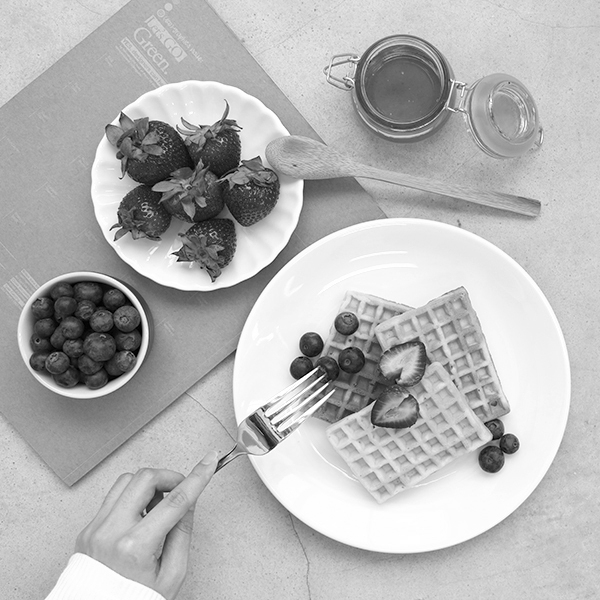
\includegraphics[width=0.9\linewidth]{images/samples/sample1.png}
    \caption*{sample1.png}
    \centering
    \end{subfigure}
    \begin{subfigure}[t]{.4\textwidth}
    \centering
    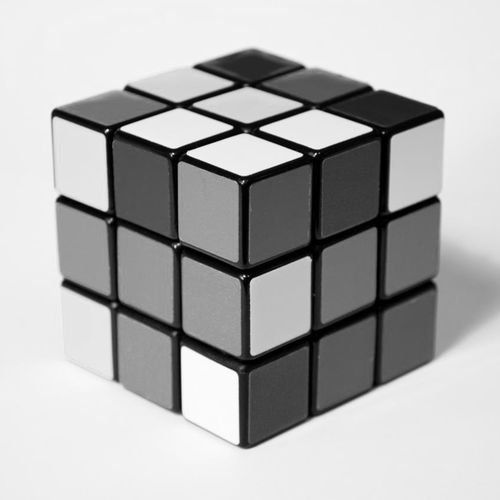
\includegraphics[width=0.9\linewidth]{images/samples/sample2.png}
    \caption*{sample2.png}
    \end{subfigure}
    \begin{subfigure}[t]{.3\textwidth}
    \centering
    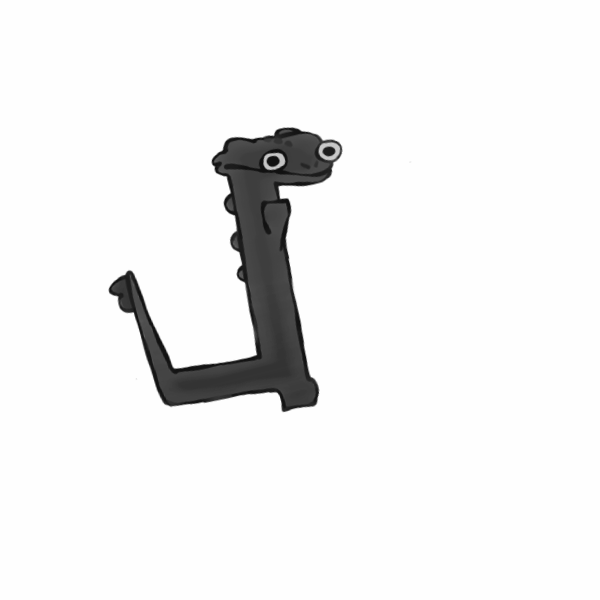
\includegraphics[width=0.9\linewidth]{images/samples/sample3.png}
    \caption*{sample3.png}
    \end{subfigure}
    \begin{subfigure}[t]{.3\textwidth}
    \centering
    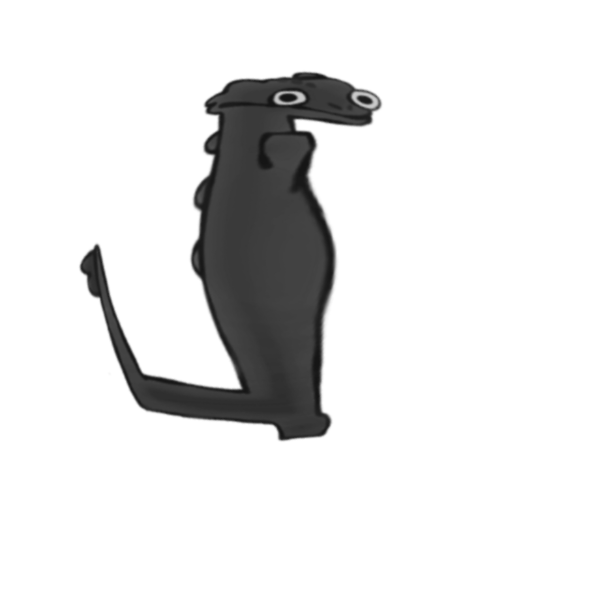
\includegraphics[width=0.9\linewidth]{images/samples/sample4.png}
    \caption*{sample4.png}
    \end{subfigure}
    \begin{subfigure}[t]{.3\textwidth}
    \centering
    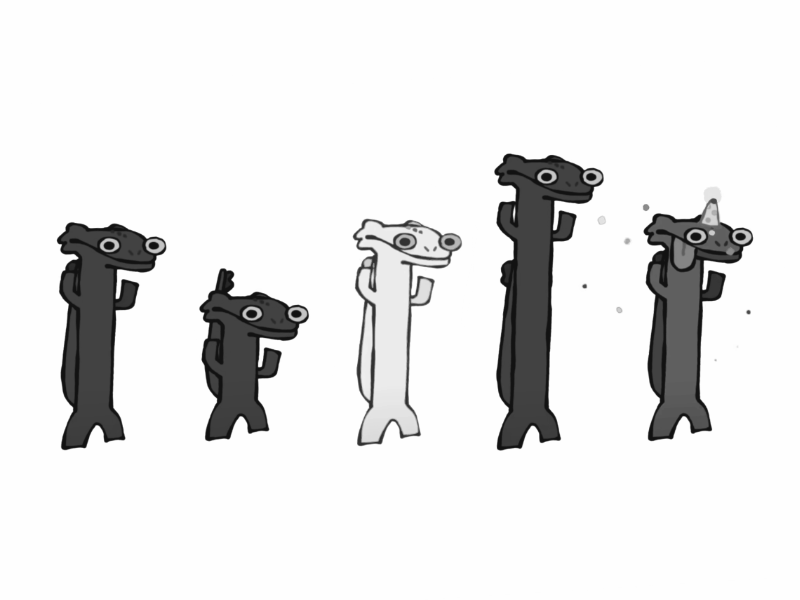
\includegraphics[width=0.9\linewidth]{images/samples/sample5.png}
    \caption*{sample5.png}
    \end{subfigure}
    \caption{這是一個全部照片的標題}
\end{figure}

\newpage
\subsection{Color Box}

\begin{tcolorbox}[title=My title]
  My box with my title.
  \tcblower
  Lower part of my box.
\end{tcolorbox}

\begin{tcolorbox}[colback=blue!5!white,colframe=blue!75!black,title=My title]
  My box with my color.
  \tcblower
  Lower part of my box.
\end{tcolorbox}

\begin{tcolorbox}
\textbf{
    Euler's Formula
} 
\textit{
    Euler's formula, named after Leonhard Euler, is a mathematical formula in complex analysis that establishes the fundamental relationship between the trigonometric functions and the complex exponential function,
}
\begin{align*}
    e^{ix} = cos(x) + i sin(x)
\end{align*}
\end{tcolorbox}

\begin{tcblisting}{colback=red!5!white,colframe=red!75!black,listing side text,
  title=Side by side,fonttitle=\bfseries}
This is a \LaTeX\ example:
\begin{equation}
\sum\limits_{i=1}^n i = \frac{n(n+1)}{2}.
\end{equation}
\end{tcblisting}

\newpage